% Adapted from the supplied latex_report_template.tex for Problem Pack Direction 4.
% The pack explicitly replaces deterministic ODE stability/adaptivity requirements.
\documentclass[11pt,a4paper]{article}
\usepackage[T1]{fontenc}
\usepackage[utf8]{inputenc}
\usepackage{amsmath,amssymb,amsthm,bm}
\usepackage[a4paper,margin=2.5cm]{geometry}
\usepackage{graphicx,booktabs,listings,xcolor,enumitem,float,caption,subcaption,array}
\usepackage[hidelinks]{hyperref}
\usepackage{algorithm,algpseudocode,mdframed,microtype}
\definecolor{lecture}{RGB}{70,130,180}
\definecolor{seminar}{RGB}{205,92,92}
\definecolor{formbg}{RGB}{250,250,245}
\definecolor{formframe}{RGB}{180,170,140}
\newmdenv[backgroundcolor=formbg,linecolor=formframe,linewidth=0.8pt,
roundcorner=3pt,innerleftmargin=8pt,innerrightmargin=8pt,
innertopmargin=8pt,innerbottommargin=8pt]{formbox}
\newtheorem{proposition}{Proposition}[section]
\algrenewcommand{\algorithmicrequire}{\textbf{Input:}}
\algrenewcommand{\algorithmicensure}{\textbf{Output:}}
\lstset{language=Python,basicstyle=\ttfamily\scriptsize,
keywordstyle=\color{blue}\bfseries,commentstyle=\color{green!40!black},
stringstyle=\color{red!70!black},numbers=left,numberstyle=\tiny\color{gray},
frame=single,breaklines=true,showstringspaces=false,tabsize=4,captionpos=b}
\captionsetup{font=small}
\setcounter{tocdepth}{1}
\graphicspath{{../figures/}}
% Replace only with confirmed information supplied by the team.
\newcommand{\TeamNumber}{NOT PROVIDED}
\newcommand{\SubmissionDate}{11 October 2026}
\newcommand{\TeamMembers}{Yifan Chen (2362353), Zeya Hu (2362375),\\
Yanle Li (2363600), Qingwen Ma (2361052), Chenyi Xu (2359968)}
% These names/IDs were transcribed from the team's latest supplied slide deck.
% Roles, individual contributions and signatures must not be invented.

\newcommand{\GBMEMRate}{0.500}
\newcommand{\GBMEMWeakRate}{0.999}
\newcommand{\GBMMilRate}{0.991}
\newcommand{\GBMMilWeakRate}{1.000}
\newcommand{\GBMAnalyticWeakRate}{0.9993}
\newcommand{\GBMFitWindow}{$N=64,128,256,512,1024$}
\newcommand{\GBMExactMean}{105.1987}
\newcommand{\GBMExactVariance}{1045.0120}
\newcommand{\GBMExactMeanCI}{[105.0403, 105.3571]}
\newcommand{\NARate}{0.491}
\newcommand{\NAFitWindow}{$N=8,16,32,64$}
\newcommand{\NAExactMean}{105.08796}
\newcommand{\NAExactMeanCI}{[104.89962, 105.27629]}
\newcommand{\NAPayoff}{14.53804}
\newcommand{\NAPayoffCI}{[14.40515, 14.67093]}
\newcommand{\NAWeakInterpretation}{The 95\% intervals include zero at $N=64,128,256$. No weak order is assigned to the complete grid range. The finest-reference payoff is estimated as 14.53804 with interval [14.40515, 14.67093].}
\newcommand{\NAReferenceInterpretation}{The last refinement discrepancy is 0.04016. It is 3.2\% to 8.9\% of the coarse strong differences on the prespecified fitting window. This meets the practical 10\% reference-sensitivity criterion used for that window. For $N=256$, the ratio is 18.0\%, so the finest coarse points are retained as sensitivity evidence, not used for the principal rate claim. The two refinements decrease the strong discrepancy; their paired payoff intervals assess whether the benchmark changes at a detectable weak scale. Neither a small refinement difference nor a zero-containing interval is a rigorous bound on the unknown continuous-time error.}

\title{\textbf{Numerical Simulation of Financial SDEs}\\[2mm]
\large Problem 4: GBM Benchmark and Non-Affine Volatility}
\author{Team \#\TeamNumber\\[2mm]\TeamMembers\\[2mm]
\small Numerical Partial Differential Equations}
\date{\SubmissionDate}
\begin{document}
\maketitle
\begin{abstract}
This report compares exact simulation, Euler--Maruyama (EM), and scalar Milstein for geometric Brownian motion (GBM), then studies a non-affine stochastic-volatility model without an exact transition sampler. All resolution comparisons share Brownian paths through aggregation of fine increments. In GBM, the measured terminal strong slopes are \GBMEMRate{} for EM and \GBMMilRate{} for Milstein, consistent with orders one half and one. Both methods nevertheless have identical first-order bias in the terminal mean. Paired estimates, independently fitted control variates, and an analytic discrete-mean identity separate this bias from sampling noise. Histograms, quantiles, moments, and positivity diagnostics supply additional checks. For the prescribed non-affine model, simultaneous log-price EM produces positive prices, and three nested numerical references yield an empirical strong slope of \NARate{} on the stated fitting window. Fine-grid call-payoff differences have confidence intervals containing zero, so no resolved weak order is claimed. Independent-seed repetitions assess variability of fitted rates, while a measured kernel-cost study compares GBM methods at a common accuracy threshold. Numerical-reference agreement and sampling intervals remain evidence rather than exact-error bounds.
\end{abstract}
\noindent\textbf{Keywords:} SDE; Euler--Maruyama; Milstein; Monte Carlo; nested grids.
\newpage
\tableofcontents
\newpage

\section{Introduction and motivation}\label{sec:introduction}
Asset prices are driven by both systematic growth and random shocks. Numerical SDE methods must therefore approximate random paths and expectations, rather than only one deterministic trajectory. We chose this direction because GBM provides an exact benchmark for checking an implementation, whereas non-affine volatility requires a numerical reference. The contrast exposes what a convergence plot can establish and what remains uncertain \cite{pack,higham,kloeden}.

\subsection{Interpreting the assignment}
The first page of the supplied problem pack explicitly specialises the generic ODE project brief for Direction~4. Exact--EM--Milstein comparison, strong and weak convergence with coupled paths, Monte Carlo uncertainty, and non-affine nested-grid validation replace deterministic stability-region and adaptive-step analyses. Consequently RK4, implicit-Euler Newton iterations, stiffness ratios, and an adaptive ODE controller are not additional tasks here. We retain the supplied report template's narrative structure, pseudocode, verification, cost comparison, references and transparency appendices.

\subsection{GBM model and exact oracle}\label{sec:gbm-model}
With initial price $S_0>0$, drift $\mu$, constant volatility $\sigma>0$, and standard Brownian motion $W$, the model is
\begin{equation}\label{eq:gbm-sde}
dS_t=\mu S_t\,dt+\sigma S_t\,dW_t,\qquad 0\le t\le T.
\end{equation}
Time is measured in years and prices in currency units; $\mu$ has units year$^{-1}$ and $\sigma$ year$^{-1/2}$. It\^o's lemma, with $f'(S)=1/S$ and $f''(S)=-1/S^2$, gives
\begin{equation}\label{eq:gbm-log}
dX_t=(\mu-\tfrac12\sigma^2)\,dt+\sigma\,dW_t,\qquad X_t=\log S_t.
\end{equation}
The exact pathwise oracle and terminal moments are
\begin{align}
S_t&=S_0\exp\{(\mu-\tfrac12\sigma^2)t+\sigma W_t\},\label{eq:exact}\\
m&=\mathbb E[S_T]=S_0e^{\mu T},\label{eq:gbm-mean}\\
v&=\operatorname{Var}(S_T)=S_0^2e^{2\mu T}(e^{\sigma^2T}-1),\label{eq:gbm-var}\\
q_p&=S_0\exp\{(\mu-\tfrac12\sigma^2)T+\sigma\sqrt T\Phi^{-1}(p)\}.\label{eq:gbm-quantile}
\end{align}
We selected $S_0=100$, $\mu=0.05$, $\sigma=0.30$, $T=1$ for GBM; the pack does not prescribe these GBM values. Equations~\eqref{eq:gbm-mean}--\eqref{eq:gbm-var} give mean $105.1271$ and variance $1040.7868$. An exact terminal value is calculated using the same $W_T$ as the numerical path, not a separate random draw.

\subsection{Prescribed non-affine model}\label{sec:nonaffine-model}
With $X_t=\log S_t$, the second model is
\begin{align}
dX_t&=[\mu-\tfrac12g(Y_t)^2]\,dt+g(Y_t)\,dW_t^{(1)},\label{eq:na-x}\\
dY_t&=\kappa(\theta-Y_t)\,dt+\xi\sqrt{1+Y_t^2}\,dW_t^{(2)},\label{eq:na-y}\\
g(y)&=\sigma_{\min}+\frac{\sigma_{\max}-\sigma_{\min}}{1+e^{-y}},\qquad
d\langle W^{(1)},W^{(2)}\rangle_t=\rho\,dt.\label{eq:na-g}
\end{align}
Here $Y$ is a dimensionless latent volatility factor, $g(Y)$ is instantaneous asset volatility, $\kappa$ is a mean-reversion rate, $\theta$ its long-run factor level, $\xi$ the factor's noise scale, and $\rho$ the instantaneous driver correlation. The bounded logistic function keeps $g$ between two positive limits. The nonlinear factor diffusion prevents using the GBM exact transition formula.
\begin{table}[H]\centering
\caption{The prescribed non-affine baseline, reproduced without changing the pack's parameters.}\label{tab:na-parameters}
\begin{tabular}{cccccc}\toprule
$S_0$ & $Y_0$ & $\mu$ & $\kappa$ & $\theta$ & $\xi$\\\midrule
100 & 0 & 0.05 & 2 & $-0.2$ & 0.6\\\midrule
$\rho$ & $\sigma_{\min}$ & $\sigma_{\max}$ & $T$ & $X_0$ & strike $K$\\\midrule
$-0.7$ & 0.10 & 0.50 & 1 & $\log100$ & 100\\\bottomrule
\end{tabular}
\end{table}
Sections~\ref{sec:methods} and \ref{sec:implementation} explain the methods and implementation. Section~\ref{sec:experiments} compares accuracy, uncertainty and cost. Section~\ref{sec:conclusions} states the limitations.
\newpage

\section{Discretisation, convergence and stochastic stability}\label{sec:methods}
\subsection{Three GBM updates}
Let $t_n=nh$, $h=T/N$ and $\Delta W_n=W_{t_{n+1}}-W_{t_n}$. Brownian motion has independent increments with
\begin{equation}\label{eq:increment}
\Delta W_n=\sqrt h Z_n,\quad Z_n\sim\mathcal N(0,1),\quad
\mathbb E[\Delta W_n]=0,\quad \mathbb E[(\Delta W_n)^2]=h.
\end{equation}
The variance is $h$, whereas the standard deviation is $\sqrt h$. Exact simulation, price-based EM and scalar Milstein are respectively
\begin{align}
S_{n+1}^{\rm exact}&=S_n^{\rm exact}\exp\{(\mu-\tfrac12\sigma^2)h+\sigma\Delta W_n\},\label{eq:gbm-exact-step}\\
S_{n+1}^{E}&=S_n^E(1+\mu h+\sigma\Delta W_n),\label{eq:em}\\
S_{n+1}^{M}&=S_n^M[1+\mu h+\sigma\Delta W_n+
\tfrac12\sigma^2((\Delta W_n)^2-h)].\label{eq:mil}
\end{align}
An update formula advances an approximation by one time step from known old values. Milstein includes $\tfrac12 b(S)b'(S)((\Delta W)^2-h)$, with $b(S)=\sigma S$ \cite{higham,kloeden}. EM on the GBM log price instead reproduces equation~\eqref{eq:gbm-exact-step} exactly; its Milstein correction vanishes. It is therefore inappropriate for demonstrating a nonzero GBM time-discretisation error.

\subsection{Strong versus weak error and convergence order}\label{sec:orders}
The terminal errors used throughout are
\begin{align}
e_s(h)&=\mathbb E|S_N^{(h)}-S_T|,\label{eq:strong}\\
e_w(h;\varphi)&=|\mathbb E[\varphi(S_N^{(h)})]-\mathbb E[\varphi(S_T)]|.\label{eq:weak-definition}
\end{align}
Strong error compares corresponding realizations; weak error compares an observable's expectation. Neither is a maximum-in-time path error. If $e(h)\sim Ch^p$ with $C>0$, then $\log e(h)\sim\log C+p\log h$, so the log--log slope approaches $p$.

For GBM, expanding the exact multiplier shows the leading term that EM omits:
\begin{equation}\label{eq:local-expansion}
e^{(\mu-\sigma^2/2)h+\sigma\Delta W}
=1+\mu h+\sigma\Delta W+\tfrac12\sigma^2[(\Delta W)^2-h]
+O_{L^2}(h^{3/2}).
\end{equation}
The centered quadratic increment has variance $2h^2$. The martingale part of the local error has centered, orthogonal increments across steps: its scale accumulates like a square root of the number of steps, rather than their absolute sum, giving $\sqrt{T/h}\,h=O(h^{1/2})$. The state-weighted errors need not be independent. Milstein cancels that leading term; its remaining local $L^2$ defect is $O(h^{3/2})$, with local mean defect $O(h^2)$, yielding a global $O(h)$ scale. This is an explanatory order argument, not a complete proof. The standard strong-convergence theorem, using globally Lipschitz coefficients and the required coefficient derivatives and finite moments, justifies EM order $1/2$ and scalar Milstein order $1$ in this GBM setting \cite{higham,kloeden}. It also implies the corresponding terminal $L^1$ upper bounds by Cauchy--Schwarz.

For the particular weak observable $\varphi(S)=S$, both schemes have the same conditional mean because the noise terms in equation~\eqref{eq:increment} are centered:
\begin{align}
\mathbb E[S_{n+1}^E\mid\mathcal F_{t_n}]&=(1+\mu h)S_n^E,\label{eq:conditional-em}\\
\mathbb E[S_{n+1}^M\mid\mathcal F_{t_n}]&=(1+\mu h)S_n^M,\label{eq:conditional-mil}\\
\mathbb E[S_N^E]=\mathbb E[S_N^M]&=S_0(1+\mu h)^{T/h}.\label{eq:discrete-mean}
\end{align}
Using $\log(1+\mu h)=\mu h-\mu^2h^2/2+O(h^3)$ gives the signed bias
\begin{equation}\label{eq:weak}
b_{\rm exact}(h)=S_0(1+\mu h)^{T/h}-S_0e^{\mu T}
=-\tfrac12 S_0e^{\mu T}\mu^2Th+O(h^2).
\end{equation}
The nonzero leading constant for our $\mu=0.05$ proves first-order mean bias. If $\mu=0$, this mean bias vanishes and there is no slope to measure. Identical mean bias does not imply identical biases for every payoff.

\subsection{Non-affine log-EM and correlated noise}
From independent $Z_{1,n},Z_{2,n}\sim\mathcal N(0,1)$, generate
\begin{equation}\label{eq:correlation}
\Delta W_n^{(1)}=\sqrt h Z_{1,n},\qquad
\Delta W_n^{(2)}=\sqrt h(\rho Z_{1,n}+\sqrt{1-\rho^2}Z_{2,n}).
\end{equation}
Both increments have variance $h$, and their covariance is $\rho h$. The simultaneous EM update is
\begin{align}
X_{n+1}&=X_n+[\mu-\tfrac12g(Y_n)^2]h+g(Y_n)\Delta W_n^{(1)},\label{eq:na-em-x}\\
Y_{n+1}&=Y_n+\kappa(\theta-Y_n)h+\xi\sqrt{1+Y_n^2}\Delta W_n^{(2)},\label{eq:na-em-y}\\
S_{n+1}&=e^{X_{n+1}}.\label{eq:na-price}
\end{align}
Both right-hand sides use $Y_n$, not the newly computed $Y_{n+1}$. We do not implement multidimensional Milstein. With $a(y)=\xi\sqrt{1+y^2}$ and $c=\sqrt{1-\rho^2}$, the diffusion columns relative to independent drivers and their commutator are
\begin{equation}\label{eq:commutator}
b_1=(g,\rho a)^\top,\quad b_2=(0,ca)^\top,\quad
(Db_2)b_1-(Db_1)b_2=(-ca\,g'(y),0)^\top\ne0.
\end{equation}
Cross terms and iterated stochastic integrals cannot in general be removed. Copying the scalar GBM correction would not justify strong order one \cite{kloeden}.

\subsection{Moment checks and positivity instead of ODE stability plots}
For GBM's price methods, the first and second expected multiplier moments are
\begin{equation}\label{eq:discrete-second}
\mathbb E[A]=1+\mu h,\qquad
\mathbb E[A_E^2]=(1+\mu h)^2+\sigma^2h,\qquad
\mathbb E[A_M^2]=\mathbb E[A_E^2]+\tfrac12\sigma^4h^2.
\end{equation}
They give finite discrete terminal moments and independent analytic checks. Growth of moments is not itself instability: the physical GBM mean and variance also grow. We do not claim unrestricted numerical stability from a lack of observed blow-up. Positivity, finiteness and reference sensitivity are separate diagnostics; Section~\ref{sec:positivity} analyses the price multipliers.
\newpage

\section{Implementation and experimental protocol}\label{sec:implementation}
\subsection{Coupled paths and the role of the grid}
A grid is the set of time points where a method updates its states. Finer grids have shorter steps and more updates per path. Let $\delta$ be the finest step and $h=r\delta$. Every coarser increment is formed by addition:
\begin{equation}\label{eq:coupling}
\Delta W_n^{(h)}=\sum_{j=nr}^{(n+1)r-1}\Delta W_j^{(\delta)}.
\end{equation}
We aggregate each driver separately, preserving its variance and driver correlation. We then rerun each method's states from the initial conditions on its own grid. We do not merely select a subset of fine-grid prices. Independent paths across grids would measure path mismatch rather than strong discretisation error.

\begin{algorithm}[H]
\caption{Coupled terminal comparison with bounded-memory batches}\label{alg:coupled}
\begin{algorithmic}[1]
\Require Model, initial data, $T$, nested grids, path count $M$, seed, batch size
\Ensure Terminal errors, paired intervals, diagnostics and saved arrays
\State Initialise a fixed-seed generator and streaming statistics
\For{each independent batch of paths}
\State Generate Brownian increments on the finest grid
\State For the non-affine model, correlate the two drivers by equation~\eqref{eq:correlation}
\For{each numerical grid}
\State Sum fine increments using equation~\eqref{eq:coupling}
\State Reset the state and apply its update rule for all time steps
\State Check finite states and collect terminal prices
\EndFor
\State Form absolute pathwise errors and signed payoff differences on paired paths
\State Accumulate moments and save the specified terminal arrays
\EndFor
\State Export CSV/JSON evidence and regenerate figures and report tables
\end{algorithmic}
\end{algorithm}

\subsection{Sampling intervals, fitted rates and control variates}
For $M$ independent observations $A_i=|S_{T,i}^{(h)}-S_{T,i}^{\rm ref}|$ and $D_i=\varphi(S_{T,i}^{(h)})-\varphi(S_{T,i}^{\rm ref})$, use
\begin{equation}\label{eq:mc-ci}
\widehat e_s=\overline A,\qquad \widehat b=\overline D,\qquad
\widehat{\rm SE}(\overline U)=\frac{s_U}{\sqrt M},\qquad
{\rm CI}_{95}(\overline U)\approx\overline U\pm1.96\frac{s_U}{\sqrt M}.
\end{equation}
Independence between paths gives the standard-error scale; the central limit theorem supplies the approximate normal interval when variance is finite. Sampling intervals are pointwise, not simultaneous, and exclude numerical-reference bias. Signed weak intervals are retained even when they cross zero. Taking the logarithm of an absolute noisy bias does not resolve its sign or justify a rate.

Production fitted rates use explicitly stated windows. Levels share paths, so an ordinary regression covariance matrix would not be an independent-level uncertainty calculation. Additional independent-seed runs in Section~\ref{sec:repeats} preserve within-run coupling and assess across-run variability instead.

The GBM mean bias is small relative to raw sampling noise. We use five exactly centered controls $C$ and a coefficient vector $\beta$ fitted on a separate pilot, then estimate $D-\beta^\top C$ in production. Conditional on the independent pilot,
\begin{equation}\label{eq:control-unbiased}
\mathbb E[D-\beta^\top C\mid\beta]=\mathbb E[D],\qquad \mathbb E[C]=0.
\end{equation}
This reduces sampling variance without substituting equation~\eqref{eq:weak} for simulated results. Appendix~\ref{app:controls} gives the control definitions; raw and controlled estimates remain in the CSV.

\subsection{Files, units and design decisions}
Algorithm~\ref{alg:coupled} explains the shared-noise workflow; Table~\ref{tab:code-files} locates its executable components.
\begin{table}[H]\centering\small
\caption{Executable components in the portable code archive. Paths are relative to its top-level folder.}\label{tab:code-files}
\begin{tabular}{lp{9cm}}\toprule
File & Purpose\\\midrule
\texttt{code/gbm.py} & Exact GBM, price EM/Milstein and independent-pilot controls\\
\texttt{code/nonaffine.py} & Simultaneous log-EM, nested grids and state diagnostics\\
\texttt{code/verify.py} & Separate recurrence/quadrature checks and saved-data consistency\\
\texttt{code/build\_report\_data.py} & Tables, numeric macros and production-report plots\\
\texttt{code/submission\_experiments.py} & Independent-seed repeat study and measured kernel-cost comparison\\
\texttt{code/run\_all.py} & One-command reproduction; isolated smoke-test mode\\\bottomrule
\end{tabular}
\end{table}
All model parameters are named constants or dictionaries; no market-data download is required. A stable logistic evaluation avoids exponentiating a large positive number. Batching controls memory but is part of reproducibility, since changing batch shape can assign pseudorandom draws to different paths. The non-affine Numba kernel accelerates time stepping but does not supply an external exact sampler. The model-specific integrator is intentionally specialised to this assignment; its constant-volatility reduction supplies a swappable special-case verification.

\begin{table}[H]\centering\small
\caption{Computational protocol; grids are nested powers of two.}
\label{tab:protocol}
\begin{tabular}{lrlr}\toprule
Quantity & Value & Quantity & Value\\\midrule
GBM production paths & 160,000 & Independent pilot & 20,000\\
GBM seed & 2026090804 & Pilot seed & 2026090805\\
GBM grids $N$ & 8 to 1024 & GBM batch & 2000\\
Non-affine paths & 100,000 & Seed & 2026090804\\
Coarse $N$ & 8,16,32,64,128,256 & Reference $N$ & 2048,4096,8192\\
GBM elapsed & 30.9 s & Non-affine elapsed & 107.8 s\\
\bottomrule\end{tabular}
\end{table}

Table~\ref{tab:protocol} records the production protocol and its measured original run costs.
The GBM rate window is \GBMFitWindow{}; the non-affine principal strong window is \NAFitWindow{}. Choices not specified in the pack include GBM parameters, path counts, seeds, grids, batch sizes, controls, fit windows and the practical 10\% reference-sensitivity screen. These choices are recorded, not presented as assignment-supplied constants. The second model's parameters are those in Table~\ref{tab:na-parameters}.
The call observable $\varphi(S)=(S-100)^+$ is an \emph{undiscounted expected payoff} under the supplied drift. It is not a risk-neutral option price without a pricing measure and discount rate.
\newpage

\section{Numerical experiments}\label{sec:experiments}
\subsection{Verification against independently constructed checks}\label{sec:verification}
The exact GBM solution in equation~\eqref{eq:exact} is our main pathwise oracle. The verification script also independently recomputes the EM/Milstein recurrences with a loop, uses Gaussian quadrature for multiplier moments, recomputes non-affine simultaneous updates in scalar Python, and reduces the non-affine model to constant volatility. In that special case log-EM must agree with exact GBM on every grid. Finally it recomputes reported strong and signed weak statistics from the saved terminal arrays. These checks test the imported executable functions rather than a disconnected explanatory listing. Recorded verification and smoke-test evidence accompany the archive. Automated checks do not constitute a signed human code review.

\subsection{GBM strong convergence}\label{sec:gbmstrong}
\begin{figure}[H]\centering
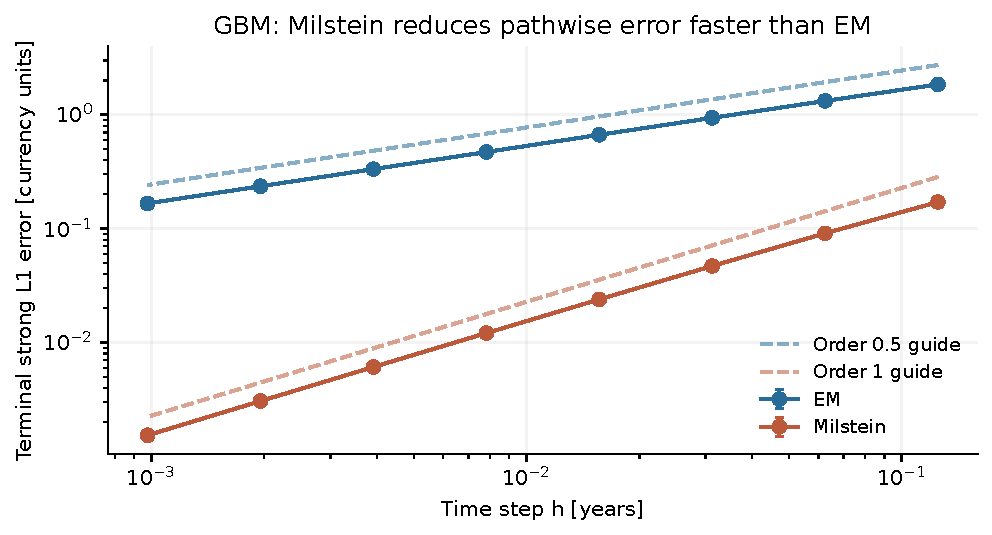
\includegraphics[width=.95\textwidth]{report_gbm_strong.pdf}
\caption{Coupled GBM terminal $L^1$ error. Reference lines benchmark orders $1/2$ and $1$; pointwise 95\% sampling intervals are often smaller than the markers. Milstein's pathwise error decays faster.}\label{fig:gbm-strong}
\end{figure}
\begin{table}[H]\centering\small
\caption{GBM strong error estimates with 95\% interval half-widths.}
\label{tab:gbm-strong}
\begin{tabular}{rrr}\toprule
$h$ & EM & Milstein\\\midrule
1/8 & $1.84750\pm0.00809$ & $0.17127\pm0.00100$\\
1/16 & $1.32218\pm0.00562$ & $0.09096\pm0.00048$\\
1/32 & $0.93847\pm0.00396$ & $0.04697\pm0.00023$\\
1/64 & $0.66641\pm0.00278$ & $0.02391\pm0.00011$\\
1/128 & $0.47071\pm0.00196$ & $0.01209\pm0.00006$\\
1/256 & $0.33297\pm0.00139$ & $0.00610\pm0.00003$\\
1/512 & $0.23550\pm0.00098$ & $0.00306\pm0.00001$\\
1/1024 & $0.16658\pm0.00069$ & $0.00153\pm0.00001$\\
\bottomrule\end{tabular}
\end{table}

Figure~\ref{fig:gbm-strong} and Table~\ref{tab:gbm-strong} give production slopes \GBMEMRate{} for EM and \GBMMilRate{} for Milstein on \GBMFitWindow{}. The distinction agrees with Section~\ref{sec:orders}. The comparison uses the same Brownian paths, not separate realizations. Exact simulation has no time-discretisation error at the grid points, although floating-point sums can change when regrouped.

\subsection{GBM weak mean convergence}\label{sec:gbmweak}
\begin{figure}[H]\centering
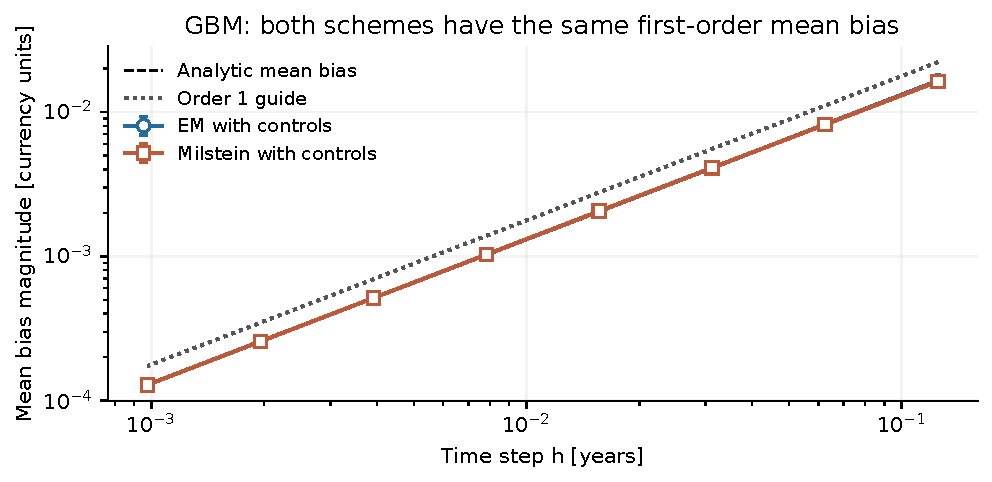
\includegraphics[width=.95\textwidth]{report_gbm_weak.pdf}
\caption{Controlled paired mean-bias estimates and the analytic discrete-mean bias. Both methods approach the same order-one line because their expected one-step multipliers coincide, not because their paths have equal accuracy.}\label{fig:gbm-weak}
\end{figure}
\begin{table}[H]\centering\small
\caption{Signed weak bias; controlled estimates plus 95\% half-widths.}
\label{tab:gbm-weak}
\begin{tabular}{rrrr}\toprule
$h$ & Analytic bias & EM controlled & Milstein controlled\\\midrule
1/8 & $-1.636\times10^{-2}$ & $-1.649\times10^{-2}$ $\pm$ $1.940\times10^{-4}$ & $-1.629\times10^{-2}$ $\pm$ $9.901\times10^{-5}$\\
1/32 & $-4.102\times10^{-3}$ & $-4.096\times10^{-3}$ $\pm$ $2.811\times10^{-5}$ & $-4.106\times10^{-3}$ $\pm$ $1.399\times10^{-5}$\\
1/128 & $-1.026\times10^{-3}$ & $-1.025\times10^{-3}$ $\pm$ $3.653\times10^{-6}$ & $-1.027\times10^{-3}$ $\pm$ $1.810\times10^{-6}$\\
1/512 & $-2.566\times10^{-4}$ & $-2.567\times10^{-4}$ $\pm$ $4.660\times10^{-7}$ & $-2.566\times10^{-4}$ $\pm$ $2.301\times10^{-7}$\\
1/1024 & $-1.283\times10^{-4}$ & $-1.284\times10^{-4}$ $\pm$ $1.649\times10^{-7}$ & $-1.283\times10^{-4}$ $\pm$ $8.144\times10^{-8}$\\
\bottomrule\end{tabular}
\end{table}

Equation~\eqref{eq:discrete-mean} explains the near-overlap in Figure~\ref{fig:gbm-weak}. The analytic fitted slope is \GBMAnalyticWeakRate{}; controlled production slopes are \GBMEMWeakRate{} and \GBMMilWeakRate{}. At $N=1024$ the analytic bias magnitude is only about $1.28\times10^{-4}$ currency units. The raw EM standard error is larger, so the archive retains both the unadjusted estimates and the variance-reduced estimates. Their independence from the pilot, rather than agreement with a desired curve alone, protects the interpretation. Table~\ref{tab:gbm-weak} compares actual estimates with the analytic oracle.

\subsection{Distribution and positivity}\label{sec:positivity}
\begin{figure}[H]\centering
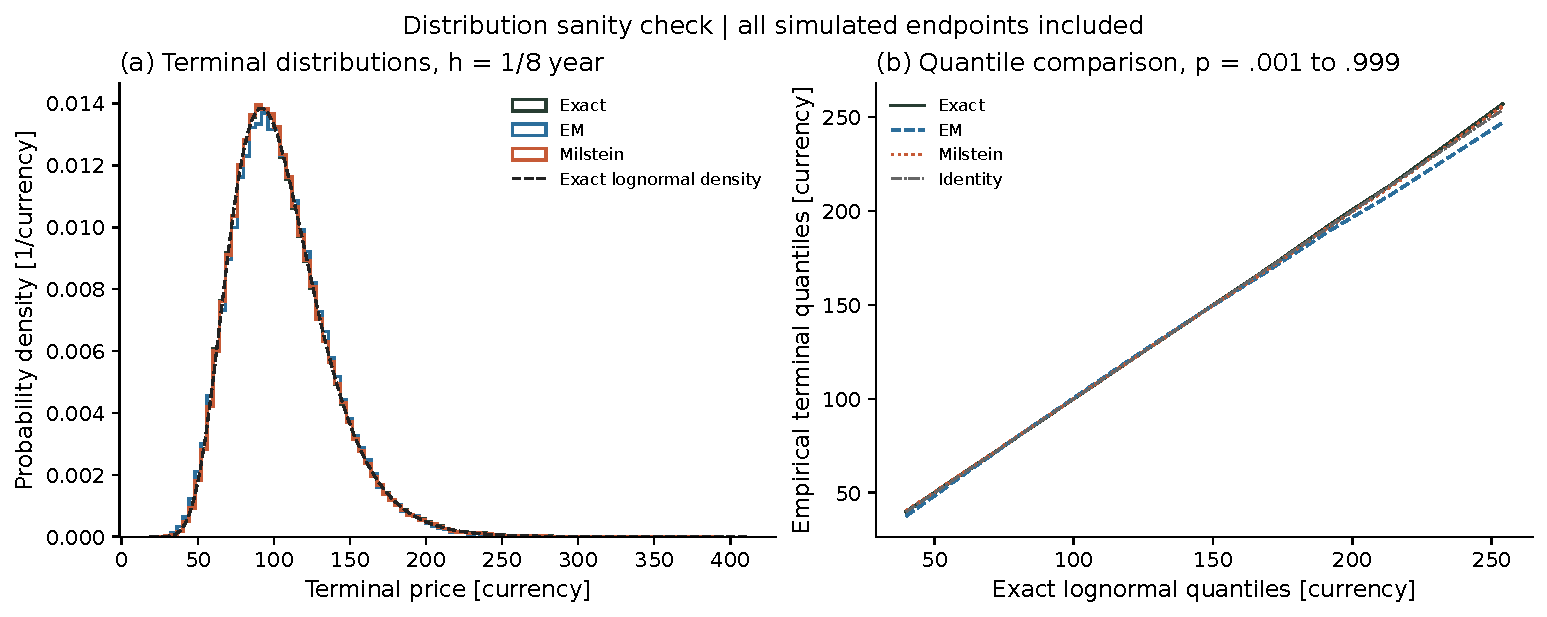
\includegraphics[width=.94\textwidth]{gbm_distribution.pdf}
\caption{GBM terminal histogram and exact lognormal density. The coarse $h=1/8$ comparison tests distributional agreement; quantiles in Table~\ref{tab:gbm-quantile} add a separate numerical check.}\label{fig:distribution}
\end{figure}
\begin{table}[H]\centering\small
\caption{Terminal quantiles; numerical columns use $h=1/8$.}
\label{tab:gbm-quantile}
\begin{tabular}{rrrrr}\toprule
$p$ & Lognormal & Exact simulation & EM & Milstein\\\midrule
0.01 & 50.012 & 49.928 & 48.387 & 50.213\\
0.05 & 61.357 & 61.378 & 60.512 & 61.615\\
0.25 & 82.091 & 82.151 & 82.303 & 82.263\\
0.50 & 100.501 & 100.557 & 101.088 & 100.582\\
0.75 & 123.041 & 123.164 & 123.653 & 123.057\\
0.95 & 164.618 & 164.485 & 163.370 & 164.043\\
0.99 & 201.961 & 202.402 & 198.376 & 201.539\\
\bottomrule\end{tabular}
\end{table}

Figure~\ref{fig:distribution} checks the density and empirical quantiles. Exact-simulation empirical mean and variance are \GBMExactMean{} and \GBMExactVariance{}, and its mean interval is \GBMExactMeanCI{}. The theoretical targets are $105.1271$ and $1040.7868$. Sampling fluctuations remain even when a sampler is exact.

For a positive old price, EM's one-step negative probability and Milstein's completed-square multiplier are
\begin{align}
\mathbb P(S_{n+1}^E<0\mid S_n^E>0)&=\Phi\!\left(-\frac{1+\mu h}{\sigma\sqrt h}\right),\label{eq:em-negative}\\
A_M&=\tfrac12\sigma^2(\Delta W+1/\sigma)^2+\tfrac12+(\mu-\tfrac12\sigma^2)h.\label{eq:mil-negative}
\end{align}
For $\sigma>0$, a negative Milstein multiplier has positive probability exactly when $(\sigma^2-2\mu)h>1$. In this baseline $\sigma^2-2\mu=-0.01$, so Milstein is positive for all $h>0$; this is not a universal statement about Milstein.
The saved terminal nonpositive counts are zero out of $160{,}000$ paths for both methods at every $N=8,16,32,64,128,256,512,1024$. These counts imply zero observed strictly negative terminals, but do not count paths ever becoming negative between terminals. Zero observations do not prove EM positivity preservation. Negative prices could distort nonlinear payoffs; clipping them would also change and bias the scheme. Neither price scheme is clipped. This optional positivity investigation is limited to formulas and terminal frequencies, not a stress-test pricing study.
\newpage

\subsection{Non-affine strong differences and reference sensitivity}\label{sec:na-strong}
\begin{figure}[H]\centering
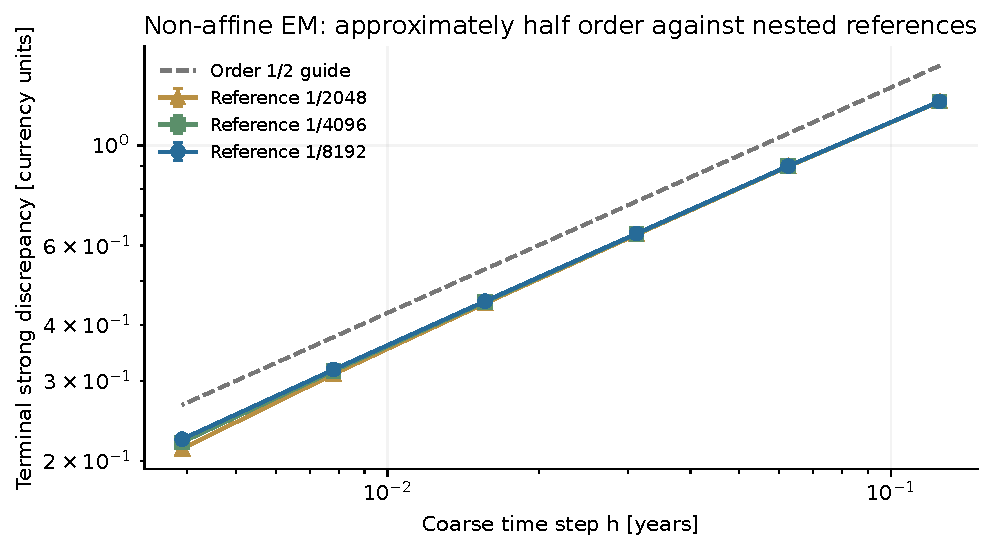
\includegraphics[width=.95\textwidth]{report_nonaffine_strong.pdf}
\caption{Terminal strong differences against three coupled numerical references. The approximately half-order slope is empirical; agreement of two EM grids is not error against an exact solution.}\label{fig:na-strong}
\end{figure}
\begin{table}[H]\centering\small
\caption{Strong discrepancy against $h_{\rm ref}=1/8192$; 95\% half-widths.}
\label{tab:nonaffine-strong}
\begin{tabular}{rrr}\toprule
$h$ & $\mathbb E|S_h-S_{\rm ref}|$ & Last reference difference / error\\\midrule
1/8 & $1.25354\pm0.00702$ & 3.2\%\\
1/16 & $0.90087\pm0.00489$ & 4.5\%\\
1/32 & $0.63818\pm0.00341$ & 6.3\%\\
1/64 & $0.45176\pm0.00241$ & 8.9\%\\
1/128 & $0.31854\pm0.00170$ & 12.6\%\\
1/256 & $0.22323\pm0.00119$ & 18.0\%\\
\bottomrule\end{tabular}
\end{table}

Against $N_{\rm ref}=8192$, the empirical slope is \NARate{} on \NAFitWindow{}. Table~\ref{tab:nonaffine-strong} records the finest-reference estimates, while Figure~\ref{fig:na-strong} displays all three references so the rate is not tied to one unexamined benchmark. The fitted slopes for references $2048$, $4096$ and $8192$ are approximately $0.496$, $0.493$ and $0.491$. Finer coarse points are more sensitive to reference resolution.
With $S^\star$ the unknown continuous-time terminal price, the reverse triangle inequality yields
\begin{equation}\label{eq:reference-bound}
\left|\mathbb E|S_h-S^\star|-\mathbb E|S_h-S_r|\right|
\le\mathbb E|S_r-S^\star|.
\end{equation}
The unknown right-hand side is not replaced by a reference-to-reference difference. We report the latter only as sensitivity evidence.
\begin{table}[H]\centering\small
\caption{Coupled refinement of the numerical reference.}
\label{tab:nonaffine-reference}
\begin{tabular}{rrr}\toprule
Refinement $N_a\to N_b$ & Strong difference & Signed payoff difference and 95\% CI\\\midrule
2048 $\to$ 4096 & $0.05679\pm0.00030$ & -0.000023 [-0.000423, 0.000377]\\
4096 $\to$ 8192 & $0.04016\pm0.00021$ & 0.000094 [-0.000188, 0.000376]\\
\bottomrule\end{tabular}
\end{table}

\NAReferenceInterpretation{}
Table~\ref{tab:nonaffine-reference} supplies the required two further reference refinements. The last strong discrepancy is about $0.04016$ currency units, with substantial impact on the finest coarse grids. The 10\% screen is a chosen practical diagnostic, not a rigorous exact-error bound.

\subsection{Non-affine weak payoff differences}\label{sec:na-weak}
\begin{figure}[H]\centering
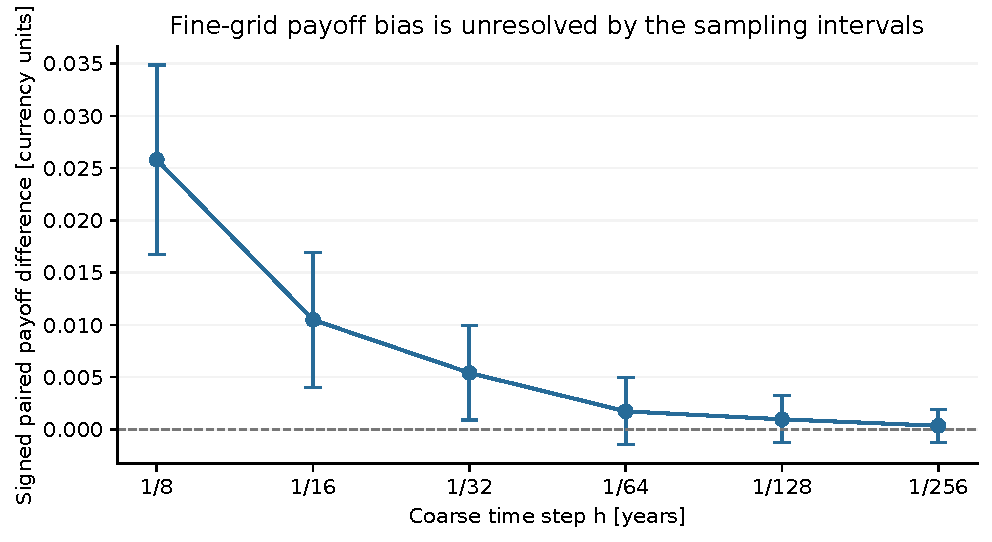
\includegraphics[width=.95\textwidth]{report_nonaffine_weak.pdf}
\caption{Signed call-payoff differences relative to $N_{\rm ref}=8192$. The zero line and paired sampling intervals show why a weak slope is not assigned to the fine-grid estimates. A signed linear ordinate avoids taking logs of intervals crossing zero.}\label{fig:na-weak}
\end{figure}
\begin{table}[H]\centering\small
\caption{Signed paired payoff differences against $h_{\rm ref}=1/8192$.}
\label{tab:nonaffine-weak}
\begin{tabular}{rrrr}\toprule
$h$ & Estimated bias & 95\% interval & Zero excluded\\\midrule
1/8 & 0.02579 & [0.01672, 0.03486] & Yes\\
1/16 & 0.01048 & [0.00405, 0.01691] & Yes\\
1/32 & 0.00540 & [0.00089, 0.00991] & Yes\\
1/64 & 0.00172 & [-0.00148, 0.00492] & No\\
1/128 & 0.00096 & [-0.00130, 0.00322] & No\\
1/256 & 0.00034 & [-0.00124, 0.00192] & No\\
\bottomrule\end{tabular}
\end{table}

\NAWeakInterpretation{}
The payoff has a corner at the strike, so smooth-test-function weak-order results cannot simply be assumed. Figure~\ref{fig:na-weak} and Table~\ref{tab:nonaffine-weak} quantify signed sampling uncertainty, not numerical-reference bias.

For the continuous model, bounded $g$ makes the stochastic exponential a true finite-horizon martingale, so the mean remains $S_0e^{\mu T}$. The discrete log-EM method preserves that same mean at any step size:
\begin{equation}\label{eq:na-mean}
\mathbb E[S_{n+1}\mid\mathcal F_{t_n}]
=S_ne^{(\mu-g(Y_n)^2/2)h}
\mathbb E[e^{g(Y_n)\Delta W_n^{(1)}}\mid\mathcal F_{t_n}]
=S_ne^{\mu h}.
\end{equation}
The Gaussian exponential expectation cancels the variance correction. Thus an accurate mean alone cannot test weak time bias for this model. This motivates a nontrivial payoff observable.

\begin{table}[H]\centering\small
\caption{Observed Brownian and state diagnostics. Increment moments are measured from generated fine increments; state checks include intermediate updates.}\label{tab:na-diagnostics}
\begin{tabular}{lrr}\toprule Quantity & Observed & Target or scope\\\midrule
Increment variance 1 & $1.221\times10^{-4}$ & $1.221\times10^{-4}$\\
Increment variance 2 & $1.221\times10^{-4}$ & $1.221\times10^{-4}$\\
Increment correlation & -0.699675 & $-0.700000$\\
Sampled increments & 4,194,304 & Predetermined first batch\\
Total path updates & 1,484,000,000 & All grids\\
Finite intermediate states & Pass & $X$ and $Y$\\
Positive finite prices & Pass & All observed states\\
\bottomrule\end{tabular}

\end{table}
The finest mean is \NAExactMean{} with sampling interval \NAExactMeanCI{}, consistent with its exact first-moment target. The expected payoff estimate is \NAPayoff{} with interval \NAPayoffCI{} for the finest \emph{discrete} model. Table~\ref{tab:na-diagnostics} checks both driver variances against $h$, correlation against $-0.7$, and finite positive asset states.
\newpage

\subsection{Independent-seed variability of fitted rates}\label{sec:repeats}
8 independent-seed GBM runs use 5,000 production paths and a separate 1,000-path control pilot each, with the same $N=64,128,256,512,1024$ fit window. 8 non-affine runs use 1,000 paths each, the same $N=8,16,32,64$ window and $N_{\rm ref}=8192$. These are additional experiments, not replacements for the 160,000- and 100,000-path production studies.\par
\begin{table}[H]\centering\small
\caption{Across-seed fitted-rate variability. Student-$t$ intervals concern the mean fitted slope under this fixed setup, not an exact theorem about the convergence order.}
\label{tab:repeat-rates}\begin{tabular}{lrrr}\toprule
Study & Mean slope & Seed SD & Approx. 95\% mean-slope CI\\\midrule
GBM EM strong & 0.5003 & 0.0083 & [0.4933, 0.5072]\\
GBM EM weak & 0.9987 & 0.0061 & [0.9936, 1.0037]\\
GBM Milstein strong & 0.9928 & 0.0032 & [0.9902, 0.9955]\\
GBM Milstein weak & 1.0003 & 0.0029 & [0.9979, 1.0028]\\
Non-affine EM strong & 0.4984 & 0.0174 & [0.4838, 0.5129]\\
\bottomrule\end{tabular}\end{table}
\begin{figure}[H]\centering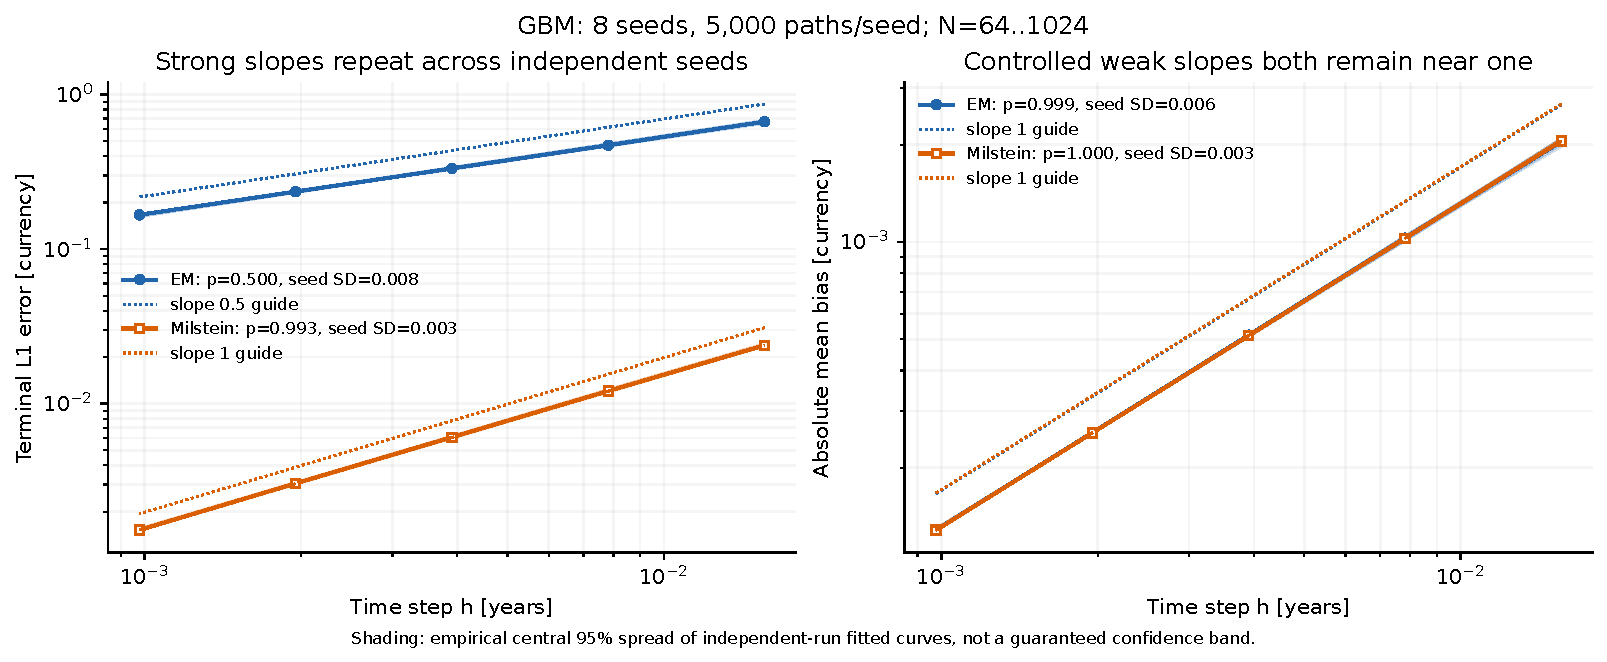
\includegraphics[width=.93\textwidth]{submission_gbm_repeat_slopes.pdf}
\caption{Independent-seed GBM fits with theoretical guides. Shading is the empirical central 95\% spread of fitted curves across runs, not an independent-level regression band or a guaranteed confidence band. Strong and weak rates remain distinct.}\label{fig:gbm-repeat}\end{figure}
\begin{figure}[H]\centering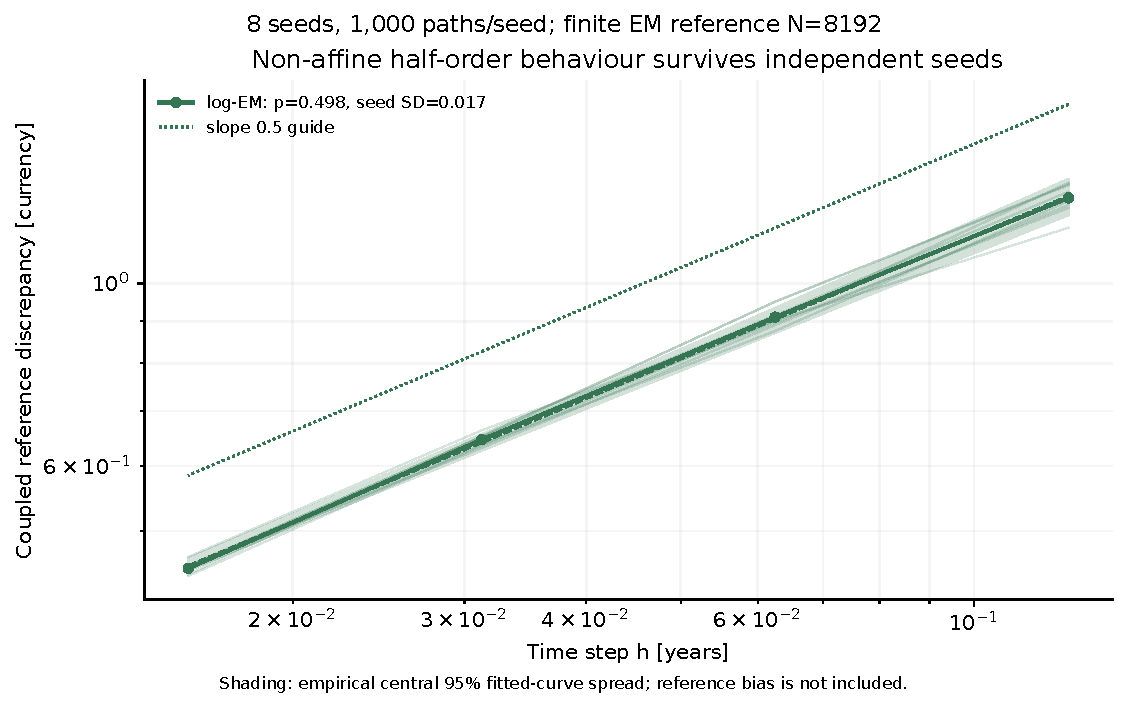
\includegraphics[width=.80\textwidth]{submission_nonaffine_repeat_slopes.pdf}
\caption{Non-affine strong fits vary across independent seeds but remain near half order for the same numerical reference. This spread does not include the unknown reference bias.}\label{fig:na-repeat}\end{figure}
Table~\ref{tab:repeat-rates} and Figures~\ref{fig:gbm-repeat}--\ref{fig:na-repeat} show the reproducibility of the fitted-rate conclusions. Only a small number of repeats is used; their empirical spread is descriptive. Coupled levels, finite fit windows and numerical references can produce systematic effects not included in a seed-only interval. In particular, Milstein's mean fitted strong slope is slightly below one and its sampling-only interval excludes one. This reflects a finite-window fitted quantity; it is not a confidence interval for the asymptotic theoretical order.



\subsection{Measured cost at a common accuracy threshold}\label{sec:cost}
Cost is measured wall-clock latency of the GBM NumPy update kernel, on the same pre-generated coupled Brownian paths after warm-up (10,000 paths; median of 7 timings). The common target is terminal $L^1$ error at most $0.25$ currency units. We select the coarsest tested grid whose upper pointwise 95\% error interval is below this target; the actual errors need not be identical, and the tolerance overshoot is reported.\par
\begin{table}[H]\centering\small
\caption{GBM kernel costs at the common accuracy target. Both methods satisfy the same threshold; their measured errors and intervals are shown rather than assumed equal.}
\label{tab:matched-cost}\begin{tabular}{lrrrr}\toprule
Method & $N$ & Error & 95\% error CI & Median cost [ms]\\\midrule
EM & 512 & 0.23566 & [0.23177, 0.23956] & 8.532\\
Milstein & 6 & 0.21605 & [0.21087, 0.22123] & 0.139\\
\bottomrule\end{tabular}\end{table}
\begin{figure}[H]\centering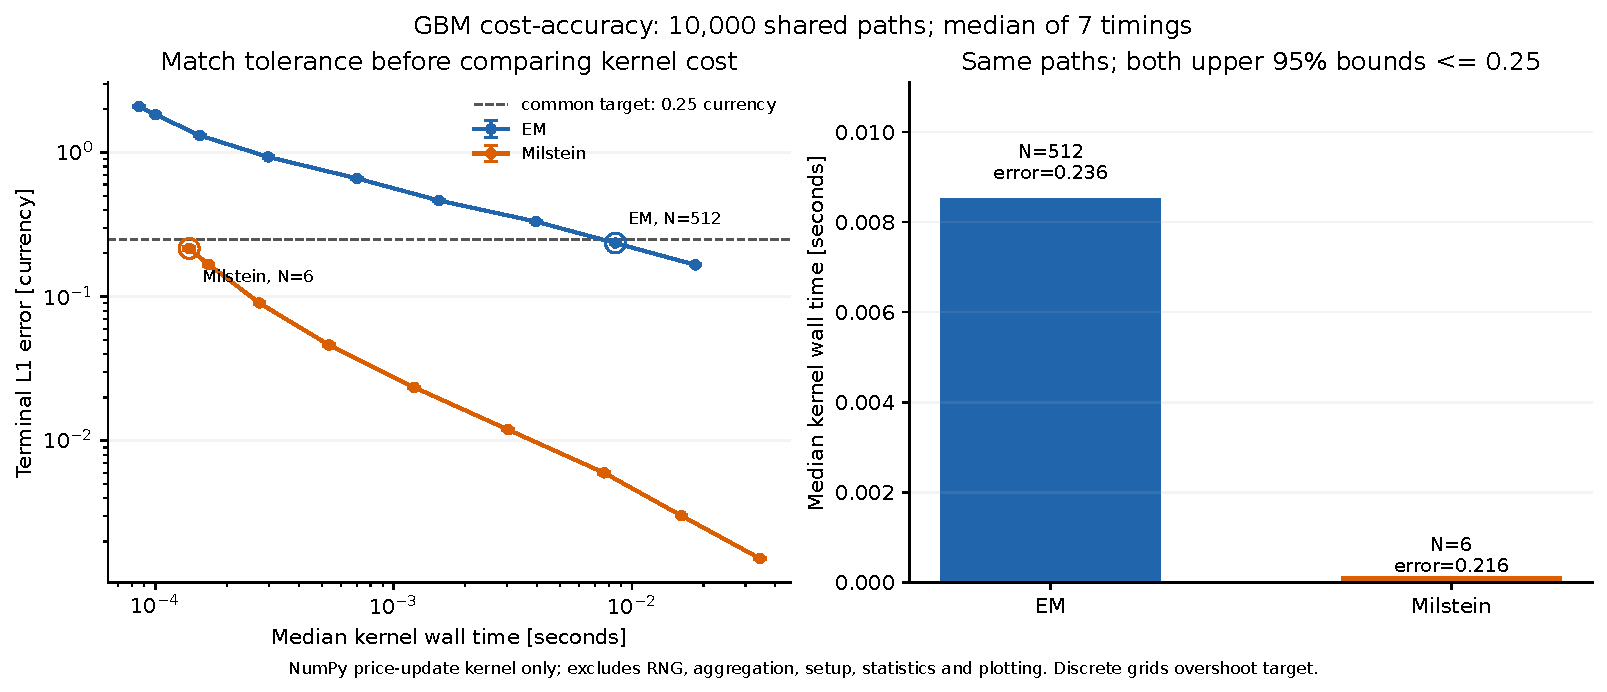
\includegraphics[width=.93\textwidth]{submission_cost_accuracy.pdf}
\caption{Measured kernel cost versus terminal strong error, using the same accuracy target and coupled paths. The target line prevents interpreting a cheap but inaccurate grid as a successful comparison.}\label{fig:cost}\end{figure}
Temporary allocations inside the price-update kernel are counted. Random-number generation, Brownian aggregation, input preparation, import/setup, compilation, statistical summaries, pilot fitting, verification and plotting are excluded from this kernel-only measure and treated consistently across methods. Raw repeated timings and the tested environment are recorded in \texttt{results/submission\_experiments.json}. The comparison in Table~\ref{tab:matched-cost} and Figure~\ref{fig:cost} therefore supports a specific implementation-level cost--accuracy conclusion, not an end-to-end runtime or cross-machine speedup.


\newpage

\section{Conclusions and limitations}\label{sec:conclusions}
GBM verifies the expected strong advantage of Milstein, but both price methods have exactly the same first-order terminal-mean bias. The observed overlap of weak curves has a mathematical explanation; it is not a plotting mistake. Exact simulation is preferable for GBM itself, while the numerical price methods provide a controlled validation exercise.

For the prescribed non-affine model, log-EM preserves positive prices and its first moment. Nested references yield approximately half-order strong differences on the selected coarse window. They do not supply an exact error. Fine-grid payoff differences are unresolved by the pointwise sampling intervals, so no complete-grid weak order is claimed.

Accuracy and work have different components. Halving the time step roughly doubles path updates; four times as many independent paths roughly halves a standard error. Coupling and controls reduce sampling noise, while refinement addresses discretisation. More paths cannot repair an underresolved reference. The supplemental cost evidence is specific to the measured implementation and stated common accuracy threshold, not a portable claim that one method is always faster.

The scope is limited to the stated parameters, horizon, terminal $L^1$ norm, path counts and fit windows. Positivity frequency diagnostics cover terminals for GBM, and all observed states for non-affine EM. We do not claim exact weak payoff errors, unconditional GBM positivity, or a scalar-Milstein rate for a noncommutative two-noise system. A useful next step is a larger paired payoff experiment with stronger reference resolution and variance reduction, followed by stress tests in higher-volatility regimes.

\subsection*{Reproducibility and intellectual ownership}
The code archive includes fixed-seed source, saved arrays, numeric results, figure-generation scripts and machine/environment evidence. It supports full reproduction and isolated reduced smoke tests. AI assistance included derivations, explanations, implementation, numerical execution and document preparation. Appendix~\ref{app:ai} records the significant claim audits and distinguishes automated verification from the team's responsibilities. Appendices~\ref{app:ics-2362353}--\ref{app:ics-2359968} record the members' individual contributions.

\begin{thebibliography}{9}
\bibitem{pack} \emph{Problem Pack: Five Suggested Directions for the ODE IVP Project}. Supplied coursework document, introductory SDE exception and Direction~4, pp.~6--7.
\bibitem{higham} D.~J. Higham. An algorithmic introduction to numerical simulation of stochastic differential equations. \emph{SIAM Review}, 43(3):525--546, 2001. \href{https://doi.org/10.1137/S0036144500378302}{doi:10.1137/S0036144500378302}.
\bibitem{kloeden} P.~E. Kloeden and E.~Platen. \emph{Numerical Solution of Stochastic Differential Equations}. Springer, 1992. \href{https://doi.org/10.1007/978-3-662-12616-5}{doi:10.1007/978-3-662-12616-5}.
\bibitem{numpy} C.~R. Harris et al. Array programming with NumPy. \emph{Nature}, 585:357--362, 2020. \href{https://doi.org/10.1038/s41586-020-2649-2}{doi:10.1038/s41586-020-2649-2}.
\bibitem{numba} S.~K. Lam, A.~Pitrou and S.~Seibert. Numba: A LLVM-based Python JIT compiler. \emph{LLVM-HPC}, 2015. \href{https://doi.org/10.1145/2833157.2833162}{doi:10.1145/2833157.2833162}.
\end{thebibliography}
\newpage
\appendix
\section{Team AI Transparency Log}\label{app:ai}
\textit{Adapted from Part A of the supplied ICS form. This is an evidence-based draft for collective confirmation, not a signed student declaration.}

\subsection*{A1. AI tools used}
\begin{table}[H]\centering\small
\begin{tabular}{p{3cm}p{4cm}p{7cm}}\toprule
Tool & Version/date & Primary use\\\midrule
OpenAI Codex & Exact model versions were not recorded. Current submission audit: 11 October 2026. & Derivations and explanations; implementation and automated verification; experiment execution; report, figures, slides and submission preparation.\\\bottomrule
\end{tabular}
\end{table}
Earlier assistance is acknowledged in the original report. Routine formatting and language edits are included in this disclosure. The team should confirm other tools or assistance it actually used. Raw conversation transcripts are not appended; they remain in the originating chat and should be exported or supplied with a content hash if requested. No transcript archive or hash is claimed here.

\subsection*{A2. Significant AI-assisted claim audits}
\begin{table}[H]\centering\small
\begin{tabular}{@{}>{\raggedright\arraybackslash}p{.8cm}>{\raggedright\arraybackslash}p{7cm}>{\raggedright\arraybackslash}p{6.8cm}@{}}\toprule
Item & Claim, assumptions and material question & Risk and possible falsifier\\\midrule
1 & Explain why the GBM EM and Milstein weak-mean curves overlap. Claim: both discrete means equal the expression in equation~\eqref{eq:discrete-mean} for deterministic initial data and independent centered Gaussian increments. & Confusing strong with weak order, omitting the centering of the Milstein term, or presenting the analytic curve as Monte Carlo output. A multiplier expectation different from $1+\mu h$ falsifies the identity.\\[2mm]
2 & Implement and interpret a numerical reference for the non-affine model: sum shared fine increments, rerun simultaneous old-$Y$ EM, and compare three reference grids. & Updating $X$ with new $Y$, using independent paths across resolutions, or calling grid differences exact errors. A constant-volatility reduction failing the exact GBM test or large reference sensitivity falsifies the implementation/interpretation.\\[2mm]
3 & Interpret empirical slopes and cost. Claim: Milstein improves strong GBM accuracy but not this mean bias; finer-grid non-affine payoff slopes are unresolved. & Treating correlated fit residuals as independent uncertainty; overlooking zero-containing payoff intervals; comparing speed at different accuracy requirements. Independent-seed spread, signed paired intervals, or matched-target cost can contradict the stated interpretation.\\\bottomrule
\end{tabular}
\end{table}

\subsection*{A3. Verification, decision and limitations}
\begin{table}[H]\centering\small
\begin{tabular}{@{}>{\raggedright\arraybackslash}p{.8cm}>{\raggedright\arraybackslash}p{7cm}>{\raggedright\arraybackslash}p{6.8cm}@{}}\toprule
Item & Separate numerical check and evidence & Decision, modification and limitation\\\midrule
1 & A direct conditional-expectation calculation in equations~\eqref{eq:conditional-em}--\eqref{eq:weak}; separate Gaussian-quadrature checks of discrete multiplier moments in \path{code/verify.py}; raw and controlled columns in \path{results/gbm_convergence.csv}. & Retain both curves. Explain their identical first-order mean bias rather than label the overlap a plot error. The statement applies to $\varphi(S)=S$ and $\mu\ne0$, not every payoff.\\[2mm]
2 & Scalar Python recurrence and constant-volatility oracle in \path{code/verify.py}; saved-array recomputation; three-grid refinements in \path{results/nonaffine_reference_checks.csv}. & Keep log-EM and simultaneous updates. Call strong rates empirical. Treat the 10\% screen as a chosen sensitivity diagnostic, not a rigorous residual bound; do not add an unjustified scalar Milstein correction.\\[2mm]
3 & Eight independent-seed repetitions and kernel-cost measurement in \texttt{code/submission\_experiments.py}; recorded JSON/CSV and plots; pointwise production payoff intervals. & Add across-run rate variability and same-target cost evidence. Withhold a fine-grid weak-order claim. Seed spread excludes numerical-reference and fit-window bias; kernel timing excludes random-number generation and other costs.\\\bottomrule
\end{tabular}
\end{table}
\noindent These are automated checks and separate implementations produced with AI assistance. They are not represented as an independent human audit. Each member must review the evidence, reproduce a relevant check and be able to explain it before signing A4.
\newpage

\subsection*{A4. Intellectual ownership declaration --- awaiting member completion}
Each member must identify their actual contribution and trusted-library interface, and sign only after confirming that they can explain and modify team-owned methods, justify claims, and explain interface assumptions without AI during the viva. The assistant does not sign or affirm this on their behalf.
\begin{table}[H]\centering\small
\begin{tabular}{p{2.6cm}p{2.4cm}p{4.8cm}p{4.4cm}}\toprule
Name & Signature/date & Actual team-owned contribution & Trusted dependency/interface\\\midrule
Yifan Chen & \textit{Not supplied} & \textit{Member to complete} & \textit{Member to complete}\\[8mm]
Zeya Hu & \textit{Not supplied} & \textit{Member to complete} & \textit{Member to complete}\\[8mm]
Yanle Li & \textit{Not supplied} & \textit{Member to complete} & \textit{Member to complete}\\[8mm]
Qingwen Ma & \textit{Not supplied} & \textit{Member to complete} & \textit{Member to complete}\\[8mm]
Chenyi Xu & \textit{Not supplied} & \textit{Member to complete} & \textit{Member to complete}\\\bottomrule
\end{tabular}
\end{table}
\noindent Relevant interfaces include NumPy normal sampling and aggregation, Numba compilation of the EM kernel, and Matplotlib figure generation. These are examples of dependencies to describe, not assigned member roles.

\subsection*{Traceability caveat}
The available Git history uses the single author label ``Apple''. It records artefact changes but does not establish which of the five students made each change. The archive includes a history snapshot for traceability. Individual statements must accurately connect contributions to files/functions/sections and genuine existing evidence; a shared commit label must not be reinterpreted as five named authors or replaced with invented retrospective commits.

% Each page is intentionally left for its named member to complete in their own voice.
% Includes both ICS.tex Part B and the additional questions from the report template.
\newcommand{\IndividualStatement}[2]{%
\newpage
\section{Individual Contribution Statement: #1}\label{app:ics-#2}
\textbf{Name:} #1\qquad\textbf{Student ID:} #2

\textbf{Role this project:} \textit{Not supplied; member to complete.}

\begin{formbox}
\textbf{The specific things I did this project (three concrete, traceable items):}
\begin{enumerate}[leftmargin=2em,itemsep=9mm]
\item \textit{Member to complete: action, file/function or report section, actual commit/evidence.}
\item \textit{Member to complete: action, file/function or report section, actual commit/evidence.}
\item \textit{Member to complete: action, file/function or report section, actual commit/evidence.}
\end{enumerate}
\end{formbox}

\textbf{The hardest conceptual obstacle and how I addressed it:}\\
\textit{Member to complete in their own words.}\par\vspace{10mm}

\textbf{An AI-assisted output I used, what I changed and why:}\\
\textit{Member to complete; cross-reference an actual audit item in Appendix~\ref{app:ai}.}\par\vspace{10mm}

\textbf{What I would do differently (one to three sentences):}\\
\textit{Member to complete.}\par\vspace{10mm}

\textbf{One thing I still do not fully understand:}\\
\textit{Member to complete honestly.}\par\vspace{10mm}

\textbf{Anything I should have asked for help with earlier (optional):}\\
\textit{Member to complete or explicitly mark not applicable.}\par\vspace{10mm}

\textbf{Signature:} \underline{\hspace{5cm}}\qquad
\textbf{Date:} \underline{\hspace{3cm}}\par
\small This uncompleted page is not a declaration of work or intellectual ownership.
}
\IndividualStatement{Yifan Chen}{2362353}
\IndividualStatement{Zeya Hu}{2362375}
\IndividualStatement{Yanle Li}{2363600}
\IndividualStatement{Qingwen Ma}{2361052}
\IndividualStatement{Chenyi Xu}{2359968}

\newpage
\section{Control-variate definitions and reproduction}\label{app:controls}
Let $W=\sum_n\Delta W_n$, $Q=\sum_n[(\Delta W_n)^2-h]$,
$R=\sum_n[(\Delta W_n)^3-3h\Delta W_n]$, and $L=e^{\sigma W-\sigma^2T/2}$. The implemented controls are
\begin{equation}\label{eq:controls}
\begin{aligned}
C_1&=L-1,& C_2&=L(W-\sigma T)/\sqrt T,\\
C_3&=L(Q-\sigma^2Th)/\sqrt{2Th},& C_4&=L(R-\sigma^3Th^2)/\sqrt{6Th^2},\\
C_5&=\frac{L[Q^2-(2Th+4\sigma^2Th^2+\sigma^4T^2h^2)]}{\sqrt8\,Th}.
\end{aligned}
\end{equation}
Gaussian exponential tilting shifts each increment's mean to $\sigma h$ and preserves its variance $h$, giving zero expectation for all five controls. Coefficients are fitted only on independent pilot paths. The analytic discrete bias remains a validation target, never a replacement for a production estimate.
\begin{lstlisting}[numbers=none,caption={Commands from the extracted code archive's top-level directory.}]
python -m pip install -r requirements.txt
python code/verify.py
python -m unittest discover -s tests -v
python code/run_all.py --smoke
python code/run_all.py
\end{lstlisting}
Full reproduction regenerates production outputs and supplemental evidence. A smoke run is deliberately too small for scientific slope claims and writes to an isolated directory. The README records exact commands, dependency ranges, historical production versions and which cost components are excluded. The supplied report PDF does not require a local LaTeX installation merely to read it.
\end{document}
